\section{Approach Overview}
\label{sec:approach}



\begin{figure}[t]
\centering
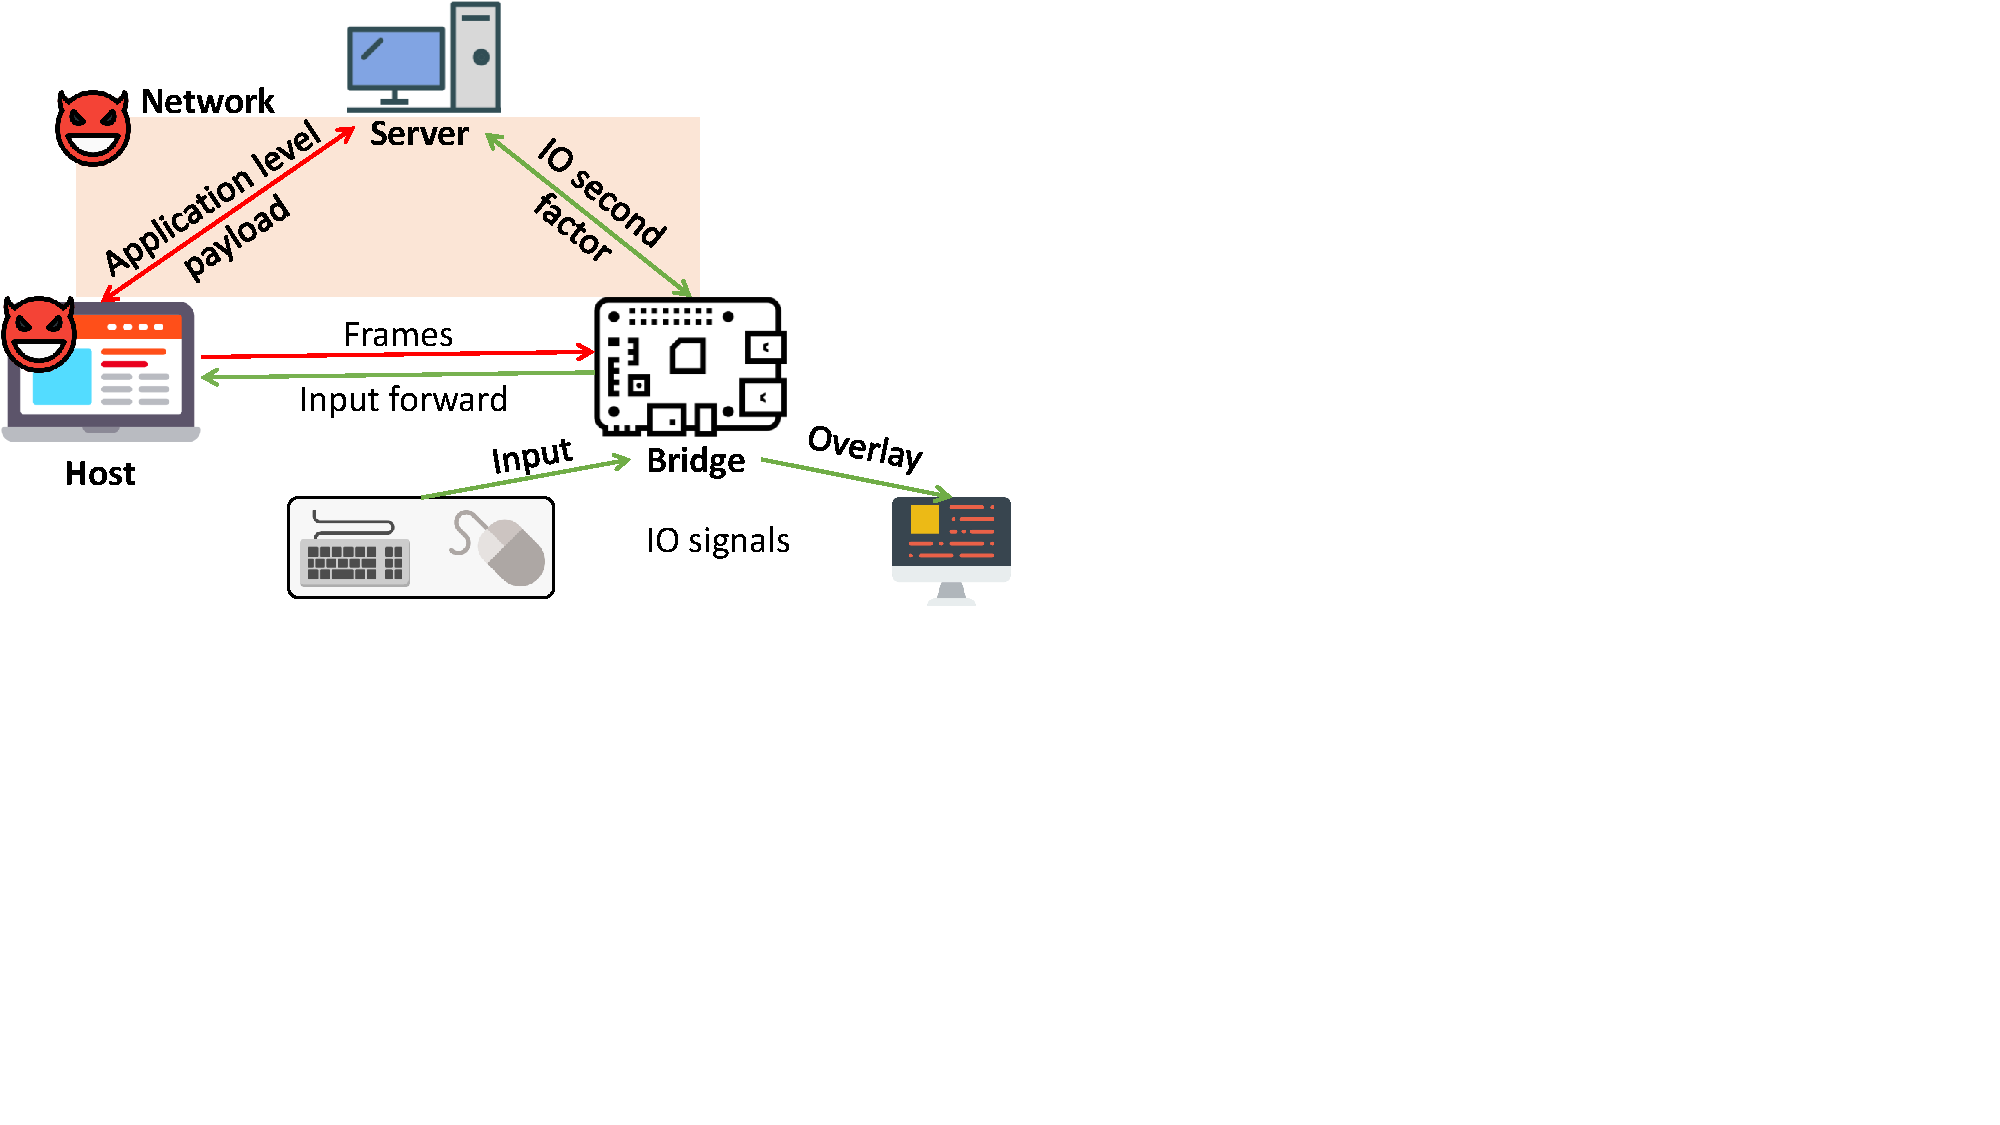
\includegraphics[trim={0 6cm 17cm 0}, clip, width=0.75\linewidth]{approachOverview.pdf}
\caption{\name: approach overview}
\label{fig:approachOverview}
\centering
\end{figure}

Given the problem statement discussed in Section~\ref{sec:problemStatement}, we first define the attacker model we consider in our proposed system.


\subsection{Attacker Model}

We assume the highly adversarial scenario where the attacker compromises the host system completely (OS, installed applications and hardware). The attacker also controlled the network. We only assume that it is a PPT-attacker, so he can not break crypto. Figure~\ref{fig:systemModel} shows the components of the system that are controlled by the attacker, i.e., the host and the network communication channel between the host and the remote server.

We only assume that the monitor, keyboard, mouse and the \device are trusted. Which is not unrealistic. The monitor, keyboard, and mouse have hardly any complex hardware. The TCB is very small.

\subsection{Challengers}

Modern user interfaces are extremely complex to analyze, and such allows many possible ways to provide input. This makes the protection of IO integrity, and privacy is a particularly challenging task. For example, given a command from the user, it is necessary to understand the user intention that corresponds to the mouse movements. Given the screen space, there exist unbounded ways for the user to move a mouse a place it on a specific UI element that fires a command to the remote end system. To provide an end-to-end protection to this entire activity one needs to 1) precisely track the cursor position, 2) correspond the cursor location to the given movement data from the mouse, 3) understand the semantics of the UI element the fires the command and 4) generate an efficient and comprehensive proof that server can use to understand the user's real intention.  


\subsection{Approach}

The overall approach is illustrated in Figure~\ref{fig:approachOverview} that utilizes a low TCB embedded device. The embedded device acts as a bridge between all IO devices and the attacker-controlled host.
